\documentclass{article} % For LaTeX2e
\usepackage{cos424,times}
\usepackage{hyperref}
\usepackage{url}
\usepackage{float}
\usepackage{graphicx}


\title{Music Genre Classification}


\author{
Abhinav Khanna\\
Student Researcher\\
\texttt{akhanna@princeton.edu} \\
\And
Amandeep Singh \\
Student Researcher \\
\texttt{email@princeton.edu} \\
}

\newcommand{\fix}{\marginpar{FIX}}
\newcommand{\new}{\marginpar{NEW}}

\begin{document}

\maketitle

\begin{abstract}
\end{abstract}

\section{Introduction}


\section{Related Work}


\section{Methods}
\subsection{Description of data}
The training data used in this paper comes from a set of 33 reference samples that have their entire genome bisulfite sequence. We primarily focus on the data for chromosome 1 for our analysis. The data consists of 33 reference samples with their methlyation proportions for each CpG site on the chromosome. Our test data consists of a sample tissue for which only a small subset of the methlyation values are accounted for. The first few columns of the training data specify the start location, the end location, and the positive or negative strand of the chromosome that the location is present on. We utilize this information to impute the values for the missing methlyation values in the test chromosome sample.

To better understand the relationships between different tissues, we computed the pearson r correlation coefficient and the corresponding p-value associated with that coefficient for each pair of tissues (Figure 2). As can be seen in table 1, certain tissues have a meaningful, non-pure chance, correlation with other tissues suggesting that certain tissues may be more apt at predicting given test values than other tissues. We also know from Figure 1 that locations that are closer together have higher correlations, and are more similar to each other than locations that are further apart on the chromosome. The finding that nearby locations have higher correlation is supported by other research in this area, such as the paper by Weiwei Zhang and Tim D Spector. 

\begin{figure}[!ht]
\begin{center}
\caption{Pearson R Correlation for neighboring index locations}
\begin{minipage}[b]{0.40\linewidth}
	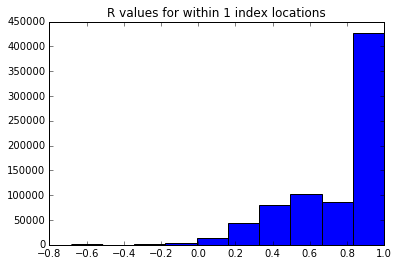
\includegraphics[scale=0.40]{CorrelationByLocation.png}
\end{minipage}
\quad
\end{center}
\end{figure}

\begin{figure}[!ht]
\begin{center}
\caption{Table of Correlation Values for Different Tissues}
\begin{minipage}[b]{0.40\linewidth}
	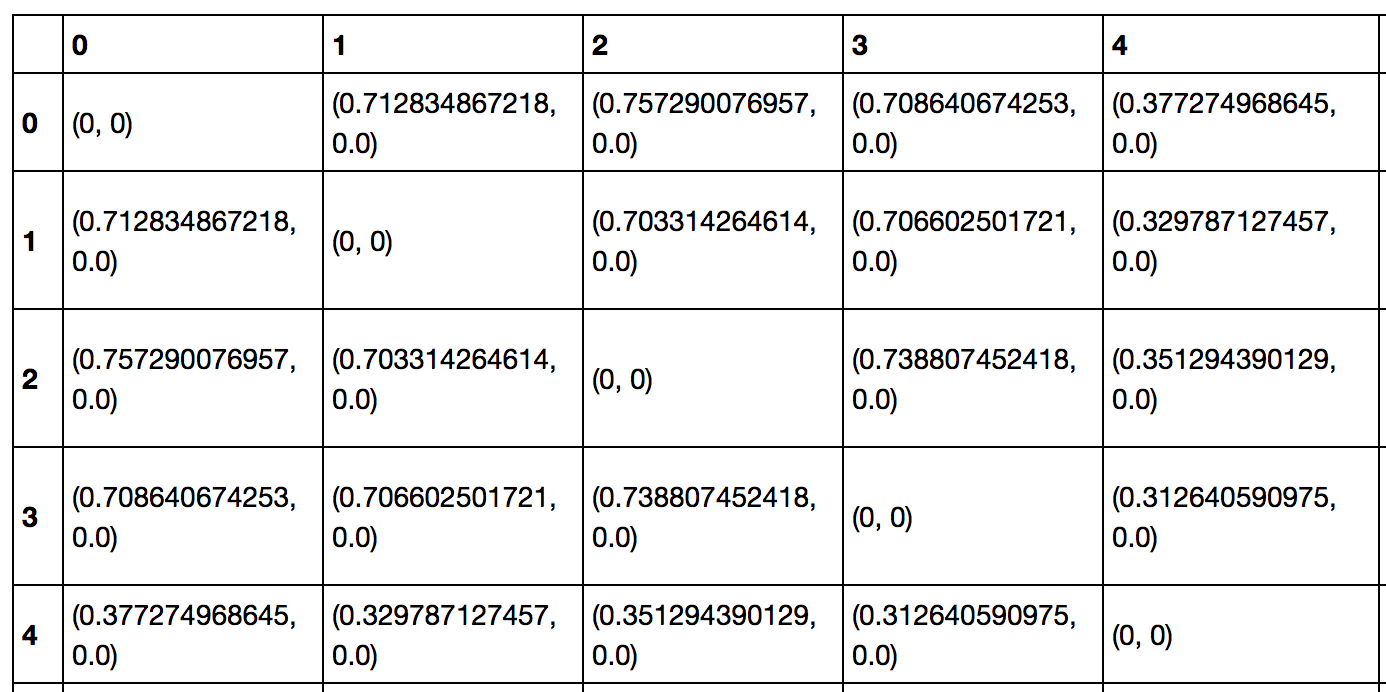
\includegraphics[scale=0.3]{table1.png}
\end{minipage}
\end{center}
\end{figure}

Examining the distribution of the mean methylation values across different tissues the distribution appears to have a right skew, and looks like it could be representative of a beta distribution. Because the mean methylation values appear like they are drawn from a beta distribution, we believe that attempting to model the similarity between our test tissue and the training tissues as a problem of judging which prior beta distribution the test sample is most likely to have been drawn from may be a worthwhile approach. The mean methylation values can be seen in Figure 2. Furthermore, plotting the methylation values across a given tissue by location yields a graph that does not look linear, suggesting that if a regressor is to be used, a non-linear one may yield better results (Figure 3).

\begin{figure}[!ht]
\begin{center}
\caption{Mean Methylation across 33 Tissues}
\begin{minipage}[b]{0.40\linewidth}
	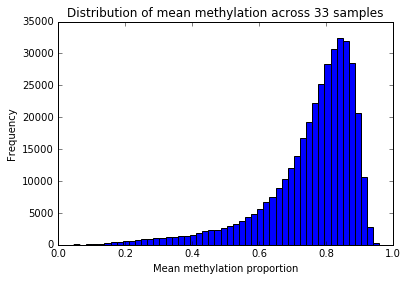
\includegraphics[scale=0.4]{MeanMethylations.png}
\end{minipage}
\end{center}
\end{figure}

\begin{figure}[!ht]
\begin{center}
\caption{Methylation Values across a Single Tissue}
\begin{minipage}[b]{0.40\linewidth}
	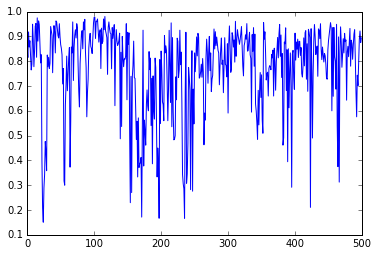
\includegraphics[scale=0.4]{GraphMethylationValues.png}
\end{minipage}
\end{center}
\end{figure}

\subsection{Imputation Pipelines}
The basic structure of our approach remained the same across pipelines. We began by calculating the similarity between the test tissue and the training tissues. The similarity was judged through some type of similarity metric, and different pipelines used different metrics. After measuring similarity, the pipelines combined the information from the most similar tissues to predict the values of the test tissue. The process of combining the information was also varied from pipeline to pipeline.
\subsubsection{Similarity Metrics Tested}
\begin{enumerate}
	\item The probability of the test vector being drawn from the beta distribution prior of a given test tissue
	\item Pearson's R correlation
\end{enumerate}

\subsubsection{Combination Methods Tested}
\begin{enumerate}
	\item Weighted mean - weights decided by similarity for some top $x$ set of similar tissues
	\item Support Vector Regression - Create SVRs for the top $x$ set of similar tissues using their training data to train the regressor on each location
	\item Decision Tree Regression
	\item Lasso Regression
\end{enumerate}

Due to time constraints, we were only able to test Pearson's R with weighted mean, and beta priors with SVRs and Decision Trees.

\subsection{Evalulation}
The effectiveness of each pipeline was judged by examining the Pearson R correlation of the filled in test vector to the full vector, computing the root mean squared error between the two vectors, looking at the residual errors, and graphing the predicted test vector against the full vector. Because we chose to only examine chromosome 1, there wasn't a great way to run cross validation testing on our prediction efforts, and without looking at the other chromosomes, we couldn't think of a way to guarantee that our methods generalize beyond chromosome 1.

\section{Results}


\section{Discussion and Conclusion}

\subsubsection*{Acknowledgments}
We would like to acknowledge Princeton University for offering the wonderful COS 424 class that provided us with the opportunity to take on this research. We would also like to thank our Professor, Professor Englehart, and her TA team for providing us with guidance and the tools necessary to make this project happen.

\bibliography{References}
\subsubsection*{References}

\end{document}
